\documentclass[10pt,conference,]{IEEEtran}
\usepackage{graphicx}
\begin{document}
\title{Spatial Rerank-based Bag-of-Words Model}

\author{\IEEEauthorblockN{Thuyen V. Phan}
\IEEEauthorblockA{Advanced Program in Computer Science\\
Faculty of Information Technology\\
University of Science, VNU - HCM\\
Email: pvthuyen@apcs.vn}
\and
\IEEEauthorblockN{Minh-Bao Truong}
\IEEEauthorblockA{Advanced Program in Computer Science\\
Faculty of Information Technology\\
University of Science, VNU - HCM\\
Email: tmbao@apcs.vn}
}

\maketitle


\begin{abstract}
The popularity of many social network sites such as Facebook, Twitter, and YouTube… creates a huge demand of managing and querying visual data from billions of images. Searching by text cannot describe the information as effective as by images but it is more complicated to search by images due to the changes of camera angles or lighting conditions. To address this problem, the authors conduct a comparison of the retrieval quality between a standard Bag-of-Words model and one with spatial reranking using RANSAC. Our experimental results on Oxford Building 5K Dataset show that spatial reranking improves the mean Average Precision of Bag-of-Words model from 0.676 up to 0.741. The authors view this work as a promising step to further improve the performance of different visual search systems using the spatial relations between the images.
\end{abstract}

\IEEEpeerreviewmaketitle

\section{Introduction} \label{section:introduction}
Alongside the intensive growth of social networks such as Facebook or Twitter, the information that users want to share is not only text but also other complex types, especially images. In January 2009, Kaplan et al. state that there are over 3 billion photos on Flickr \cite{Kaplan201059}. And in 2012, it is recorded that 250 million photos are uploaded to Facebook everyday \cite{1}. This fact creates a huge demand of managing and querying data from huge amount of information in different formats (text, image, video, sound \ldots).

The tendency to search not only by text but also some special features of other complex types such as images is currently one of the most popular concerns. Thus, huge search engines such as Google and Bing have already developed and integrated their visual search system using images as queries. Nevertheless, the problem of improving performance of visual search systems remains an interest of many research lab and corporation.

To query visual data using a single image, one of many approaches is template matching method, i.e. a technique for finding small parts of an image which match a template image \cite{brunelli_template_matching}, \cite{Rosenfeld4309663, Gharavi913587}. Another popular technique is to evaluate the similarity of two images by comparing some regions which seem to be the interested points of the images, namely features matching \cite{Belongie710790, Rubner, Viola990517}. The algorithm that the authors choose to discuss in this paper is Bag-of-Words (BoW) \cite{3} which is used by many different image retrieval systems \cite{3, 2, 7}. A reason why Bag-of-Words is widely used is that its allow parts of a query image to appear flexible in the result images. Hence, BoW model is a really potential approach and is focused by many research groups.

However, due to the flexibility among parts of the query images, BoW might not fully exploit the spatial relations among the components of images. This fact motivates our investigation to prove that cooperating the spatial information can increase the precision of BoW model. Our experiments performed on Oxford Building 5K Dataset shows that using an extra spatial rerank step has a huge impact on the BoW model in term of mean Average Precision (an increase from 0.676 to 0.741). This work's main contribution is the proof that spatial information is really useful when retrieving visual information and promote the research of enforcing spatial consistency to image retrieval systems.

The rest of this paper is organized as follows. In section \ref{section:background_relatedworks}, we review the background and related words in image retrieval and image classification. The core steps of the BoW model and how we conduct experiments are presented in section \ref{section:method}. Section IV is for experiment results and evaluations. The conclusion and future works are presented in section V.



\section{Background \& Related works} \label{section:background_relatedworks}
There are many approaches to create Image Information Retrieval System. Some methods aim at high precision, i.e achieve high quality of top retrieved results, others focus on high recall, i.e retrieve all positive results. Among them, the first effective and scalable method is Bag-of-Words, Sivic and Zisserman \cite{3}, which is inspired by the correspondence algorithm using in text retrieval. Before going into details of BoW model in subsection \ref{section:background_bow}, we will first introduce some different methods for image retrieval problem in subsection \ref{section:background_dif_method}.

\subsection{Different approaches for image retrieval problem} \label{section:background_dif_method}
One of many popular method is histogram comparisons which compares 2 different images based on their color histograms. Some early works of this approach using a cross-bin matching cost for histogram comparison can be found in \cite{Shen1983187, Werman1985328, Peleg192468}. In \cite{Peleg192468}, Peleg et al. represent images as sets of pebbles after normalization. The similarity score is then computed as the matching cost of two sets of pebbles based on their distances.

Another well-known technique is template matching, i.e. seeking a given pattern in a image by comparing to candidate regions of the same size in the target image. By consider both the pattern and candidate regions as a length-$N$ vector, we can compare these two vectors by using different kind of distance metrics, one such metric is the Minkowski distance \cite{Ouyang5770267}.

\subsection{Bag-of-Words}\label{section:background_bow}

Since Bag-of-Words is originally a text retrieval algorithm, we will first introduce some backgrounds about BoW in text retrieval problem in subsection \ref{section:bow_text} before discussing about using BoW in image retrieval in subsection \ref{section:bow_image}.

\subsubsection{Bag-of-Words in text retrieval}\label{section:bow_text}
In text retrieval, a text is represented as a histogram of words, also known as BoW \cite{4}. This scheme is called term frequency weighting as the value of each histogram bin is equal to the number of times the word appears in the document.
Moreover, some words are less informative than others since those words appear in almost every document. Therefore, we need a weighting scheme that address this problem. Such weighting scheme is called inverse document frequency (idf) and is formulated as $log(N_{D} / N_{i})$, where $N_{D}$ is the number of documents in the collection and $N_{i}$ is the number of documents which contains word $i$. The overall BoW representation is thus weighted by multiplying the term frequency (tf) with the inverse document frequency (idf) giving rise to the tf-idf weighting \cite{4}. In addtion, extremely frequent words, ``stop words'', can be removed entirely in order to reduce storage requirements and query time.


\subsubsection{Bag-of-Words in image retrieval} \label{section:bow_image}
When applying BoW to image retrieval, a major obstacle is the fact that text documents are naturally broken into words by spaces, dots, hyphens, or commas. In contrast, there is no such separator in images. Therefore, the concept of ``visual word'' is introduced where each visual word is represented as a cluster obtained using k-means on the local descriptor vectors \cite{3}.

The bigger the vocabulary size is, the more different the visual words are. Hence, the vocabulary helps us distinguish the images more effectively. Nonetheless, with bigger vocabulary size, slightly different descriptors can be assigned to different visual words thus not contributing to the similarity of the respective images and causing a drop in performance examined in \cite{5, 6, 7}. Philbin et al. \cite{7} suggests ``soft assign'' method where each descriptor is assigned to multiple nearest visual words instead of using ``hard assignment'', i.e only assign a local descriptor to only one nearest visual word. Despite its effectiveness, this method also significantly costs more storage and time.


\subsection{Evaluation the performance of image retrieval system} \label{section:evaluation_ir_sys}

Since there are many different algorithms lying behind different information retrieval systems, it is crucial to have a measurement for evaluating the performance of information retrieval systems. In this subsection, we will describe different popular measurements which are used to estimate performance of an information retrieval system. First of all, the authors would like to introduce 3 things that are required to evaluate information retrieval systems: a document collection, a set of queries, and a set of relevant documents for each query.

The 2 early born and fundamental measures are precision and recall. While precision is calculated as the ratio between the number of relevant documents that are retrieved and the total number of relevant documents, recall is the quotient between the number of relevant documents retrieved and the number of relevant documents. The formula of these 2 measures are shown below:

\begin{equation}
recall = \frac{number\;of\;relevant\;items\;retrieved}{number\;of\;relevant\;items\;in\;collection}
\end{equation}

\begin{equation}
precision = \frac{number\;of\;relevant\;items\;retrieved}{total\;number\;of\;items\;retrieved}
\end{equation}

Despite their simplicity, precision and recall fail to take into account of the order of retrieved documents which is also important since a user want to find his/her desired document as fast as possible. Therefore, many other measures, which also consider the arrangement of the retrieved documents, are developed based on precision and recall. There is one such measure named Average Precision (AP), the average value of the precision value achieved from the top documents cut-off at positions where relevant documents are retrieved. In addition to precision, recall, and AP, there are also many other measures such as F-measure, i.e. weighted average of precision and recall or R-precision, i.e. the precision at R-th position where R is the number of relevant documents.

In our experiments, to evaluate the result, the authors choose to use the AP measure along with the mean value of AP overall queries, namely mean Average Precision (mAP). Besides the fact that these 2 measures can fully evaluate both the content and the order of the ranked list, their popularity are also a reason why the authors choose them. AP and mAP are also used in many previous works in image retrieval, so we can easily compare our framework's performance with others based on these 2 measures.


\section{Method} \label{section:method}
\subsection{Overview of an Image Retrieval System}

As described in Figure \ref{fig:image_retrieval_system}, a typical Image Retrieval System consists of 2 main steps: Feature Extraction and Similarity Matching. We will explain how we do the Feature Extraction step in this section. In section \ref{section:similarity_extraction}, the authors focus on describing how we perform Similarity Matching with our implementation of BoW model.

To extract features from images, the authors choose to use Hessian affine detector \cite{Mikolajczyk2004}. As we tested on Oxford Building 5K Dataset \cite{oxbuilding}, there are typically 3,300 features for each image and a total about 16 millions of features for the whole dataset. Then, we compute the SIFT descriptors \cite{Lowe2004} of all the features and use these descriptors for the next steps.

\begin{figure}
    \centering
    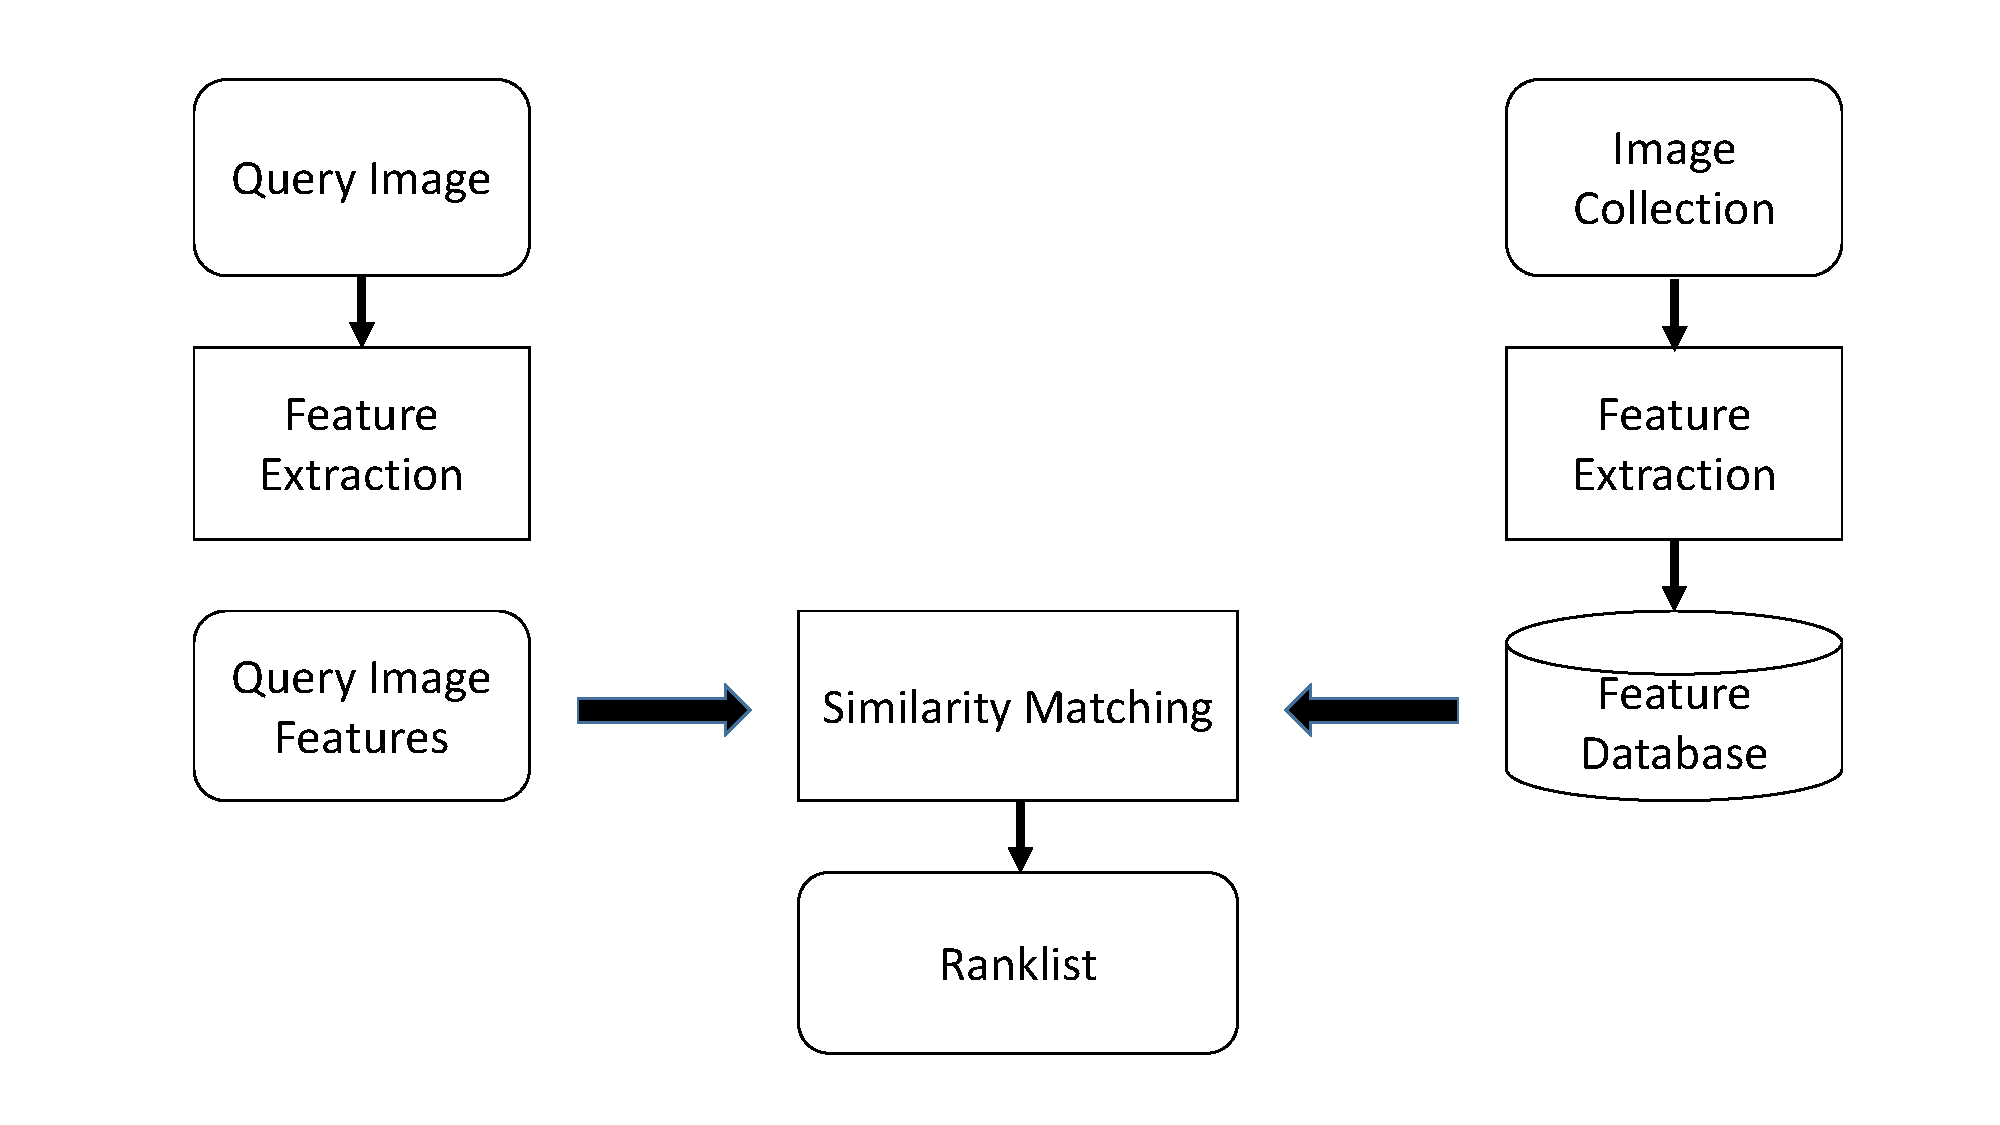
\includegraphics[width=3.0in]{ImageRetrievalSystem.pdf}
    \caption{How an image retrieval system works}
    \label{fig:image_retrieval_system}
\end{figure}

\subsection {Similarity Matching} \label{section:similarity_extraction}

As showed in Figure \ref{fig:bow_model} typical BoW model used in image retrieval systems would consist of the following steps: Dictionary Building, Quantization and Retrieving the result. The 2 former steps are described in section \ref{section:dictionary_building} and section \ref{section:quantization}. The last step is our main focus in this paper and is discussed in section \ref{section:tfidf_weighting} and section \ref{section:spatial_rerank}.

\begin{figure}
    \centering
    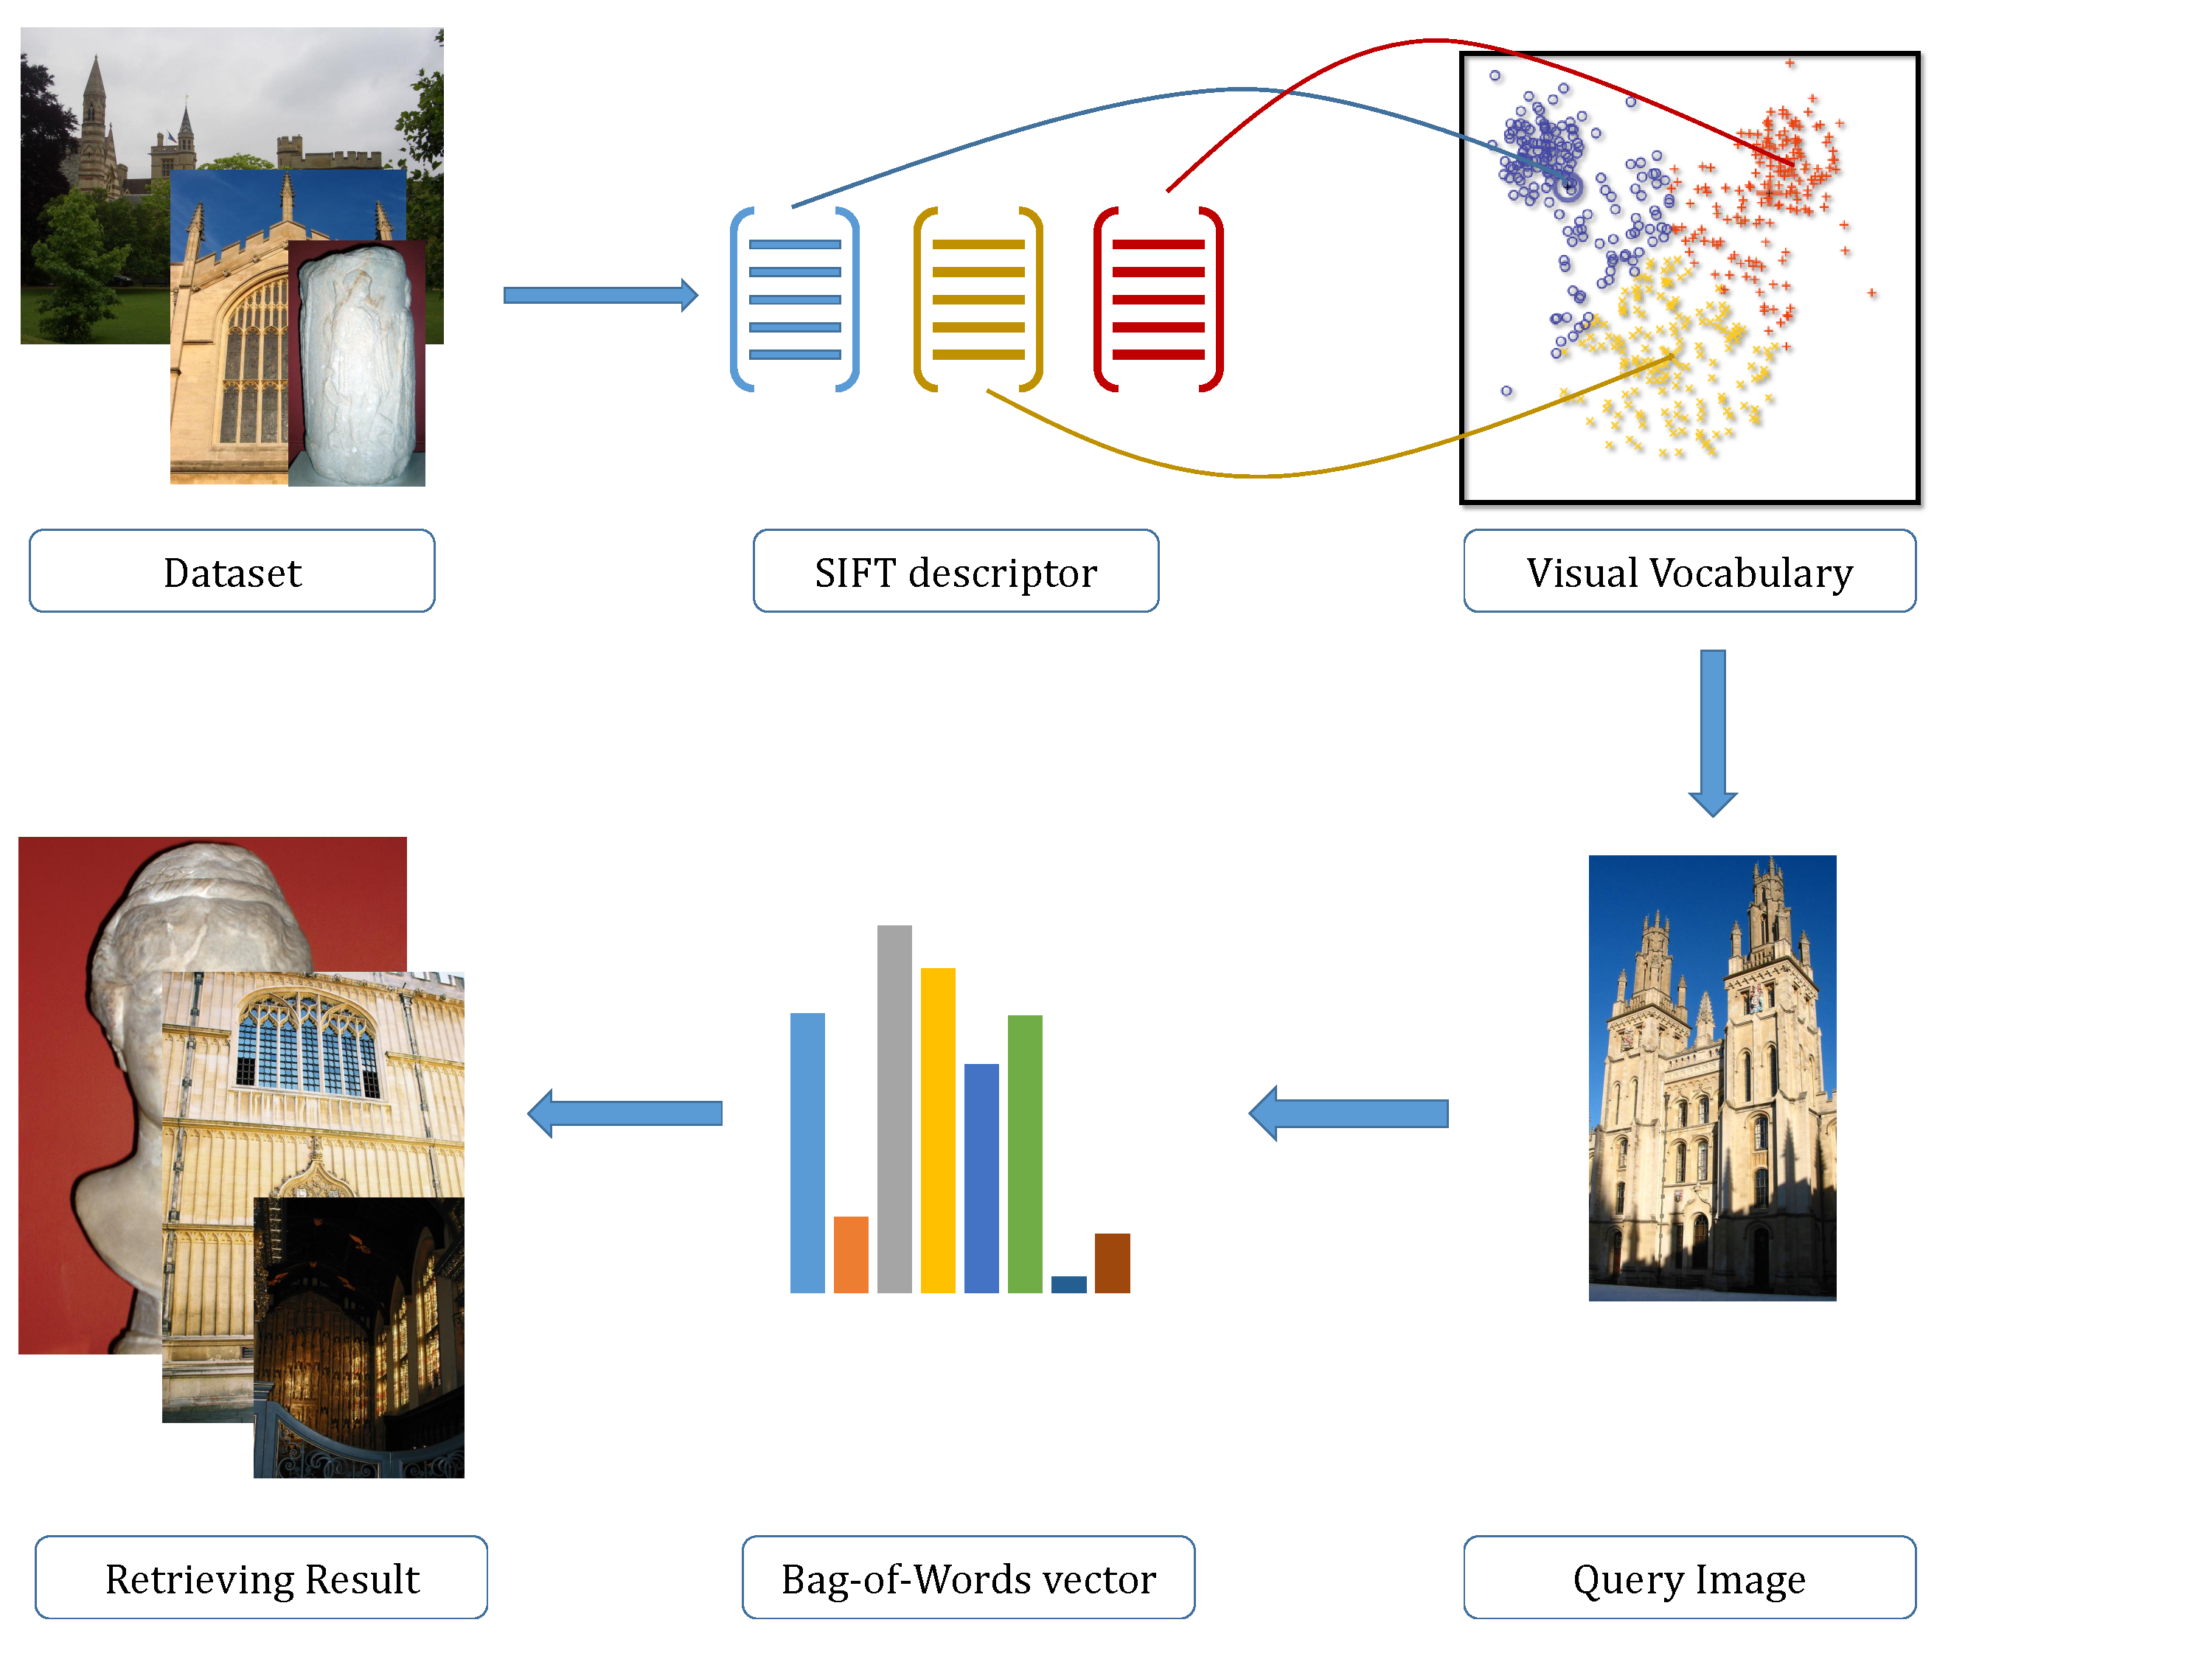
\includegraphics[width=3.0in]{process.pdf}
    \caption{Diagram of Bag-of-words model}
    \label{fig:bow_model}
\end{figure}

\subsubsection{Dictionary Building} \label{section:dictionary_building}

Generating the dictionary of visual words for such a huge amount descriptors is a big challenge. In order to overcome this obstacle, the authors use the approximate k-means (AKM) instead of the traditional exact k-means (KM). AKM is proposed by Philbin et al. \cite{2}, which reduce the majority amount of time taken by exact nearest neighbors computation by using an approximate method instead. Also, in \cite{2}, Philbin et al. shows that using 1M dictionary size would have the best performance on the Oxford Building 5K Dataset \cite{oxbuilding}.

\subsubsection{Quantization} \label{section:quantization}

Subsequently, each 128-dimension SIFT descriptor is reduced to a 3-dimension vectors of their 3 nearest visual words in the dictionary. Each of these 3 nearest cluster is assigned with weights calculated with the formula proposed by Sivic et al. \cite{7}, $weight = \exp(-\frac{d^2}{2\delta^2})$, where $d$ is the distance from the cluster center to the descriptor point and $\delta^2$ is chosen to be 6250. Then, by adding all these weights to their corresponding bins, we will have the BoW representation of an image.

\subsubsection{tf-idf Weighting Scheme} \label{section:tfidf_weighting}

As mentioned in section \ref{section:background_relatedworks}, tf-idf is a popular weighting scheme that is used by almost any BoW model. In this section, the authors will show how this scheme is applied to our system.

For a term $t_{i}$ in a particular document $d_{j}$, its term frequency $tf_{i, j}$ is defined as follow:

\begin{equation} 
        tf_{i, j} = \frac{n_{i, j}}{\sum\limits_{k} n_{k, j}}
\end{equation}
Where $n_{i, j}$ is the number of occurrences of the considered term $t_{i}$ in the document $d_{j}$. The denominator is the sum of the number of occurrences of all the terms in document $d_{j}$.

The inverse document frequency $idf_{i}$ of a term $t_{i}$ is computed by the following formula:

\begin{equation}
        idf_{i} = \log{\frac{\left|D\right|}{\left|\{j: t_{i} \in d_{j}\}\right|}}
\end{equation}
Where, $\left|D\right|$ is the total number of documents in the corpus, $\left|\{j: t_{i} \in d_{j}\}\right|$ is the number of documents where the term $t_{i}$ appears, i.e. $n_{i, j} \ne 0$

The tf-idf weight of a term $t_{i}$ in a document $d_{j}$ is then calculated as the product of tf and idf:

\begin{equation}
{tfidf}_{i, j} = tf{i, j} \times idf_{i}
\end{equation}

The tf-idf weight is then used to compute the similarity score between an image $d_{i}$ and a query $q$:

\begin{equation}
s_{d_{i}, q} = \vec{{tfidf}_{i}} \cdot \vec{{tfidf}_{q}} = \sum\limits_{j = 1}^{\left|T\right|} {tfidf}_{i, j} \times {tfidf}_{q, j}
\end{equation} 

Finally, by sorting the list of images corresponding to their similarity score with a query, we achieve the raw ranked list of this query which is then used for the Spatial Rerank step.

\subsubsection{Spatial Rerank} \label{section:spatial_rerank}

So far, we have always consider an image as a document of visual words, which means that we totally ignore the spatial structure of the features. Thus, we now incorporate the spatial constraints to the top ranked result and rerank them. The spatial verification process evaluate a geometry transformation based on features coordinates of a image and the query. The target images are then reranked using the sum of the spatial verified visual words' idf. A common approach is to use RANSAC \cite{Fischler1981}, i.e. generating different transformation hypotheses and choose the hypothese which has the largest number of ``inliers''. In our system, we perform spatial rerank on the top 800 retrieved result of the dataset, which is showed to obtain the best accuracy by Philbin et al. \cite{2}.

\section{Experiment \& Result} \label{section:experiment_result}

To prove our hypotheses, the authors test both the BoW systems with and without spatial rerank on the Oxford Building 5K Dataset \cite{oxbuilding}. This dataset was constructed by Philbin et al. in 2007 \cite{2}. It consists of 5,062 images of resolution $1024 \times 768$ belongs to 11 different Oxford buildings. Images for each building are collected from Flickr by searching using text queries. In figure \ref{fig:oxbuilding}, some samples from the dataset are shown. Along with the dataset, there are also 55 queries along with their ground-truth, 5 for each landmark, as shown in figure \ref{fig:oxbuilding_query}. The reason why the authors use this dataset is because of its popularity, it is used by many previous works in this field. Thus, we can easily compare our systems with those previous works.

\begin{figure}
    \centering
    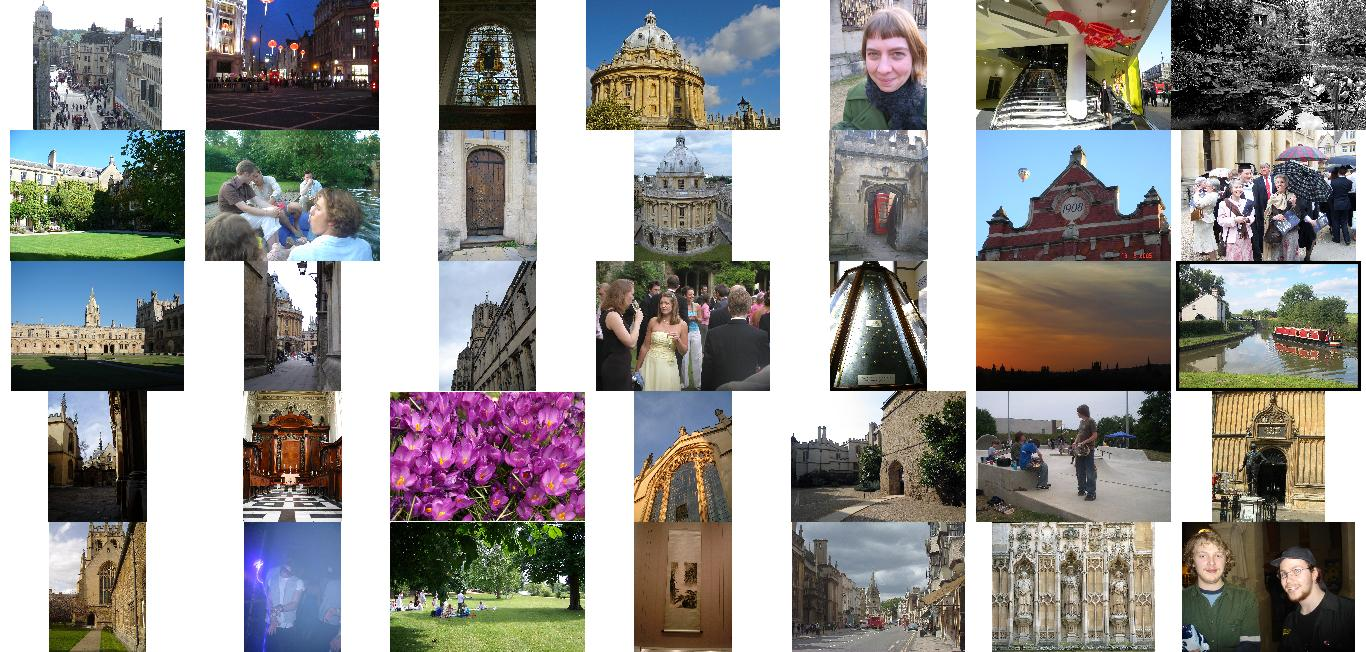
\includegraphics[width=3.0in]{oxbuilding.jpg}
    \caption{Some random images from Oxford Building 5K Dataset}
    \label{fig:oxbuilding}
\end{figure}

\begin{figure}
    \centering
    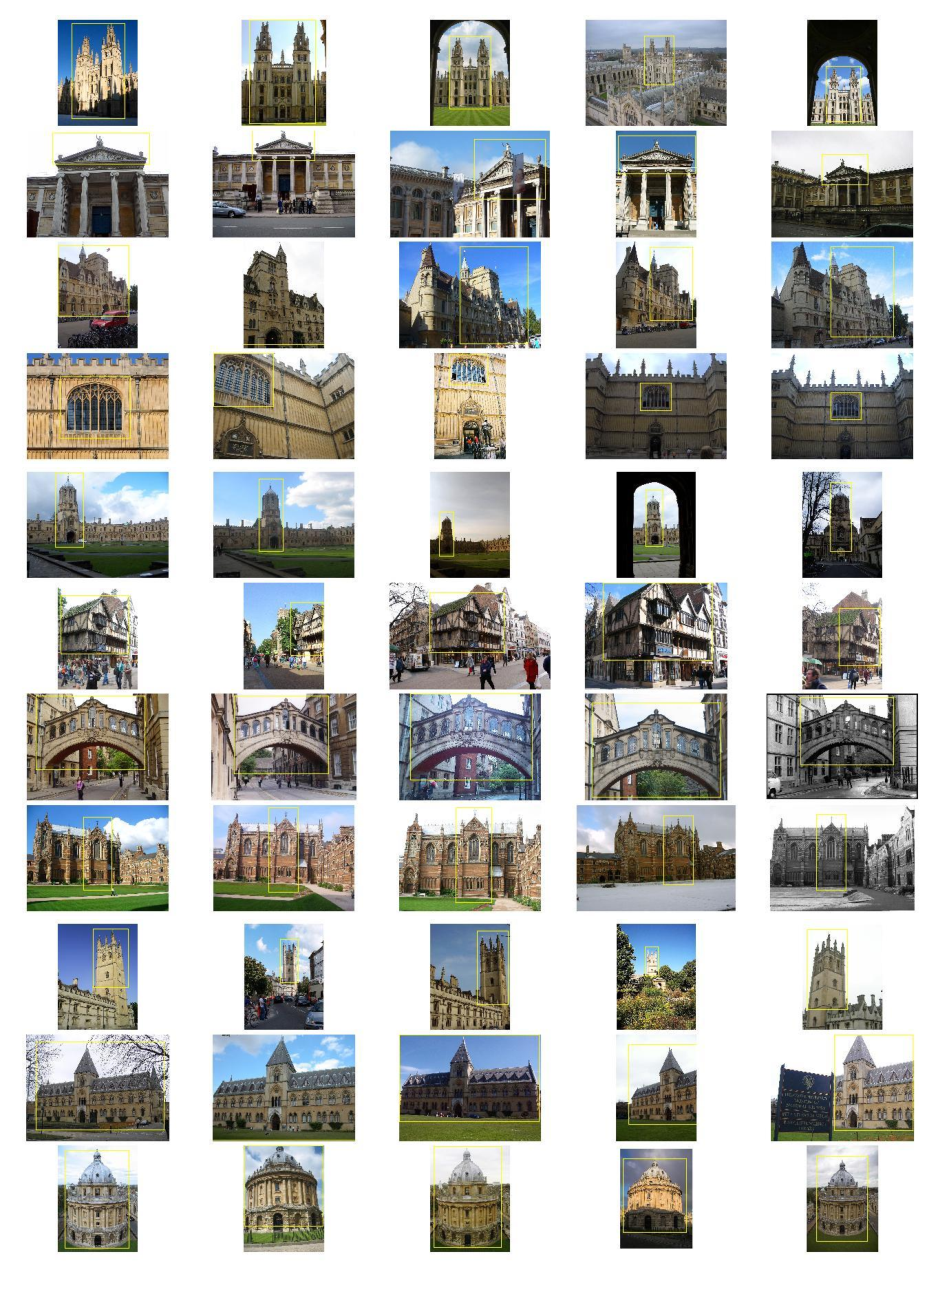
\includegraphics[width=3.0in]{oxbuilding_query.pdf}
    \caption{55 queries of Oxford Building 5K Dataset}
    \label{fig:oxbuilding_query}
\end{figure}

Our experiment shows that spatial rerank has significant impact on the retrieval quality of BoW model, an increase from 0.676 to 0.741 in term of mAP. More specifically, 74.2\% of the queries' AP are improved, the largest increment is from 0.417 to 1.000, the rest of queries approximately remain unchanged. The AP of all 55 queries are shown in figure \cite{fig:ap_chart}.

\begin{figure}
    \centering
    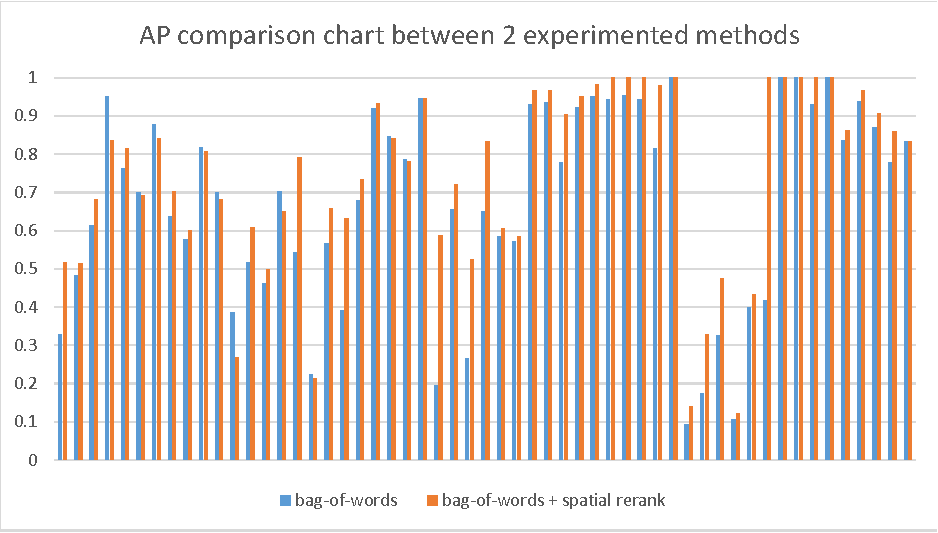
\includegraphics[width=3.0in]{mAP.pdf}
    \caption{Comparison chart between the 2 methods}
    \label{fig:ap_chart}
\end{figure}

\section{Conclusion}

Through our experiments, it is proved that spatial rerank significantly boost the performance of BoW model. This is a very potential result to further improve the performance of many image retrieval systems. In the future, we plan to keep upgrading our system to operate on other datasets which are larger in size and also more variant in term of content. Our final goal is to deploy our system for real-time usage with limited computer resources.

\bibliographystyle{IEEEtran}
\bibliography{IEEEabrv,thuyen}

\end{document}


